Consider the data on snow removal in Exercise 3.20.
\begin{enumerate}[label= (\alph*)]
    \item Comment on any possible outliers in a scatter plot of the original variables.
    
    The scatter plot of the data is below for 25 observations. There's a couple observations with large snow durations. Observation 5 and observation 21 with snow direations of 19.5 hours and 17.5 hours, respectively. Observation 21 also has a high number of work hours to clear the snow (42.3 hours).

    \begin{center}
        \begin{figure}[H]
            \centering
            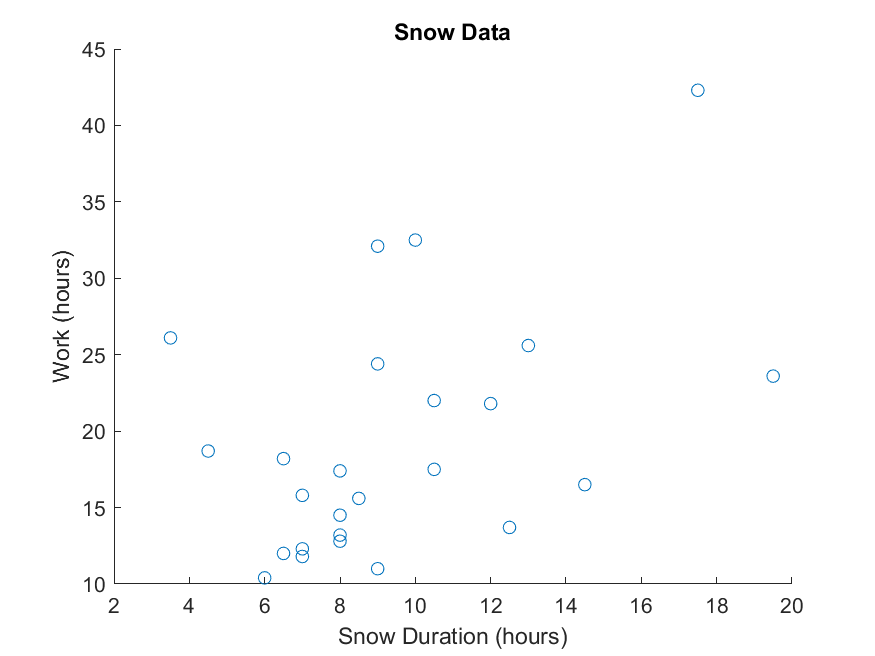
\includegraphics[scale=0.6]{./matlab/chapter-4/sol4.41.a.png}
        \end{figure}
    \end{center}

    \item Determine the power transformation $\hat{\lambda}_{1}$ the makes the $x_{1}$ values approximately
    normal. Construct a Q-Q plot of the transformed observations.

    For the snow duration in hours, $x_{1}$, the optimal Box-Cox power transformation value found was $\hat{\lambda}_{1} = 0.0501$.
    I rounded that to 0, so $x_{1}^{\prime} = x_{1}^{\hat{\lambda}_{1}} = \ln\{x_{1}\}$. This transformation increased the Q-Q correlation coefficient to 0.9872, which is larger than the critical point values of 0.9406, 0.9591, and 0.9665 who represent the 0.01, 0.05, and 0.10 levels, respectively, for a sample size of 25.
    Because of this the data would be considered normally distributed at all the usual levels.
    Below are the results of the power transformation and the Q-Q plots of the transformed data.
    The Q-Q plot of the transformed data looks pretty good.

    \begin{center}
        \begin{figure}[H]
            \centering
            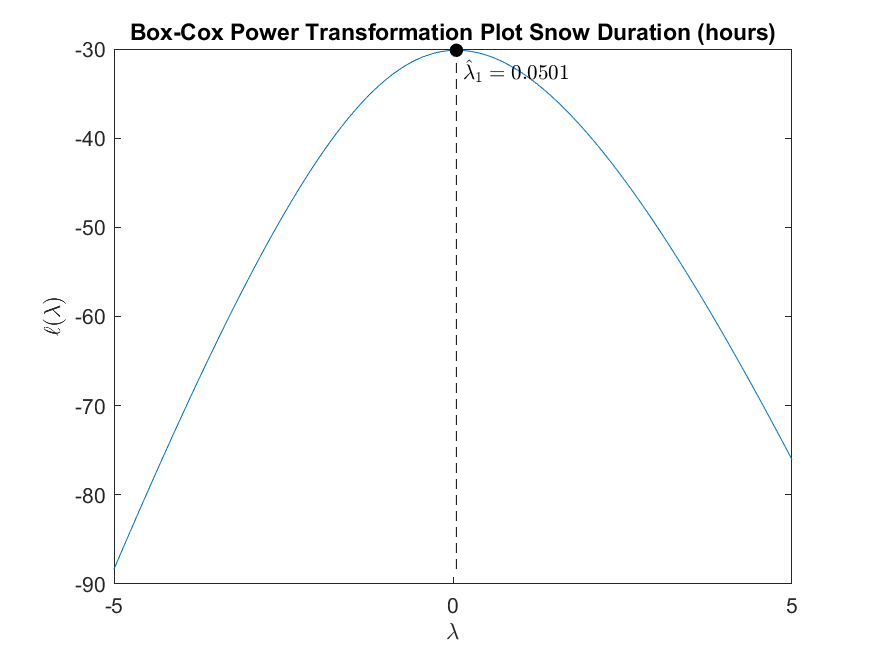
\includegraphics[scale=0.4]{./matlab/chapter-4/sol4.41.power.1.png}
        \end{figure}
    \end{center}
    
    \begin{center}
        \begin{figure}[H]
            \centering
            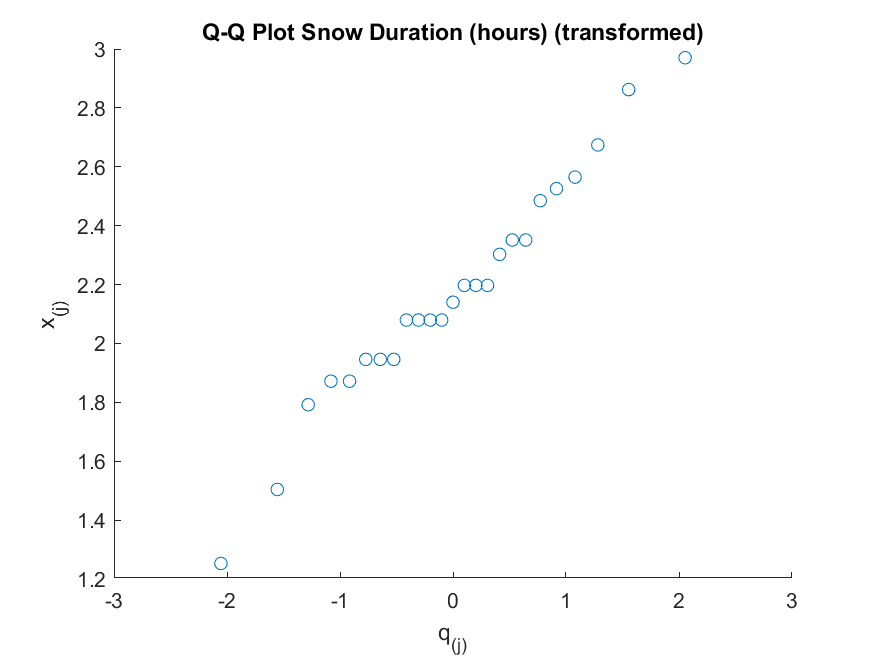
\includegraphics[scale=0.4]{./matlab/chapter-4/sol4.41.qq.tr.1.png}
        \end{figure}
    \end{center}

    \item Determine the power transformation $\hat{\lambda}_{2}$ the makes the $x_{2}$ values approximately
    normal. Construct a Q-Q plot of the transformed observations.

    For amount of time it took to clear the snow in hours, $x_{2}$, the optimal Box-Cox power transformation value found was $\hat{\lambda}_{2} = -0.6914$.
    I rounded that to -0.70, so $x_{1}^{\prime} = x_{2}^{\hat{\lambda}_{2}} = x_{2}^{-0.70}$. This transformation increased the Q-Q correlation coefficient to 0.9909, which is larger than the critical point values of 0.9406, 0.9591, and 0.9665 who represent the 0.01, 0.05, and 0.10 levels, respectively, for a sample size of 25.
    Because of this the data would be considered normally distributed at all the usual levels.
    Below are the results of the power transformation and the Q-Q plots of the transformed data.
    The transformed Q-Q plot has the linear appearance we'd hope for.

    \begin{center}
        \begin{figure}[H]
            \centering
            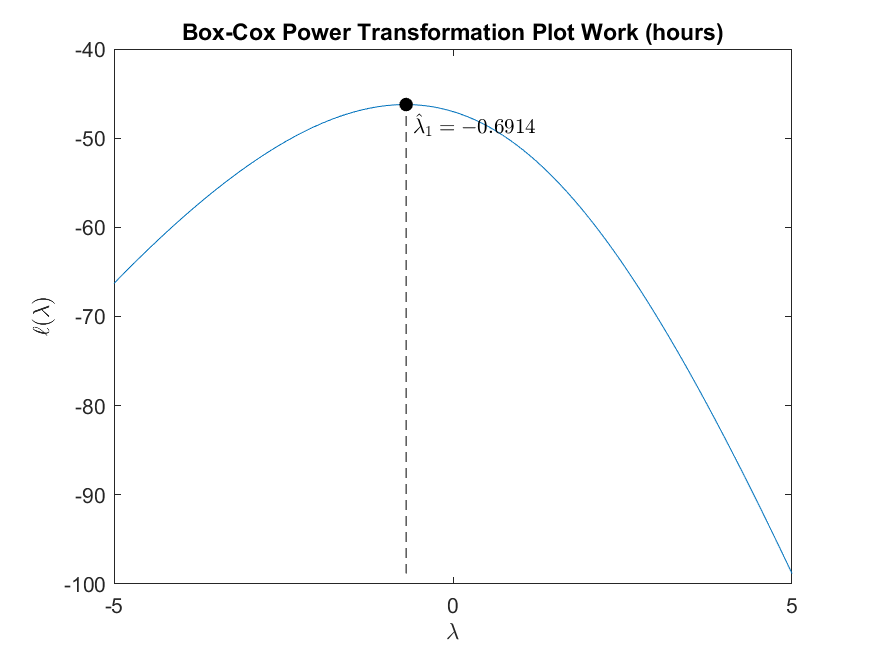
\includegraphics[scale=0.4]{./matlab/chapter-4/sol4.41.power.2.png}
        \end{figure}
    \end{center}
    
    \begin{center}
        \begin{figure}[H]
            \centering
            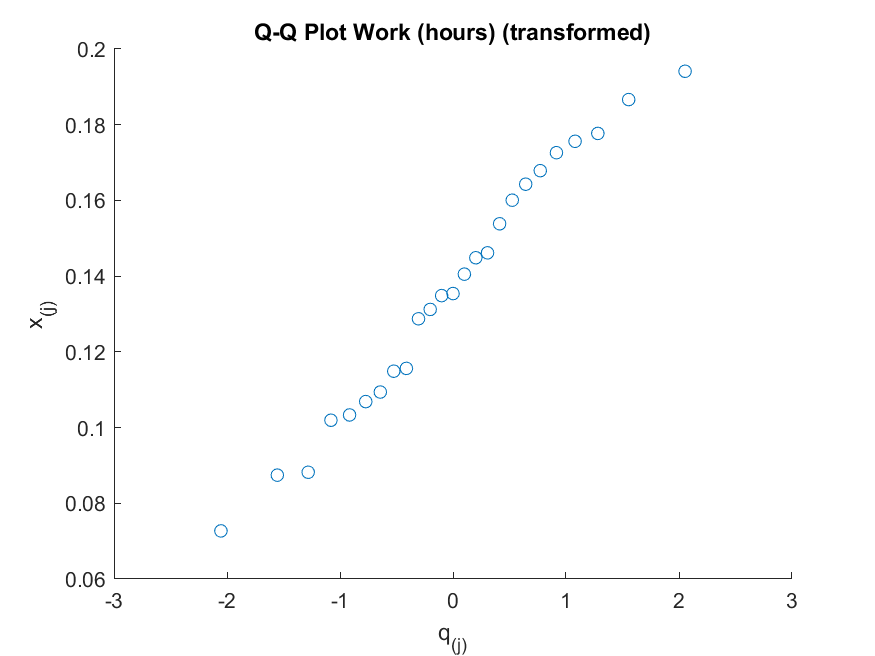
\includegraphics[scale=0.4]{./matlab/chapter-4/sol4.41.qq.tr.2.png}
        \end{figure}
    \end{center}

    \item Determine the power transformation for approximate bivariate normality using (4--40).
    
    The optimum found was at $\left(\hat{\lambda}_{1}, \hat{\lambda}_{2}\right) = (0.2349, -0.6376)$. These values are sort of close to those found in part (b) and (c), at least for $\hat{\lambda}_{2}$ anyway, where the result of optimizing the univariate transform using Box-Cox was $\left(\hat{\lambda}_{1}, \hat{\lambda}_{2}\right) = (0.0501, -0.6914)$. The contour and surface plot for $\ell \left(\lambda_{1}, \lambda_{2}\right)$ is below.

    \begin{center}
        \begin{figure}[H]
            \centering
            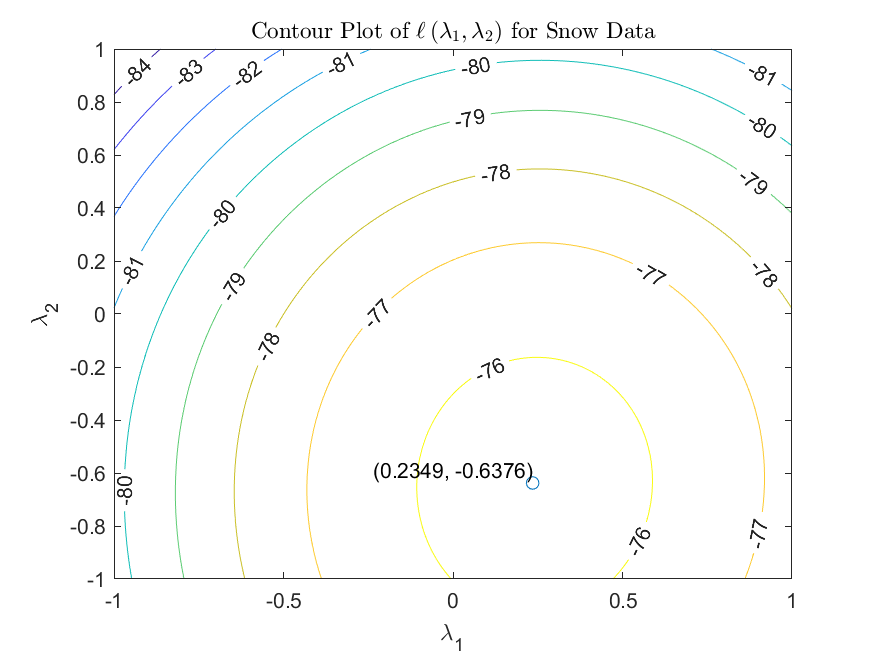
\includegraphics[scale=0.6]{./matlab/chapter-4/sol4.41.d.contour.png}
        \end{figure}
    \end{center}
    
    \begin{center}
        \begin{figure}[H]
            \centering
            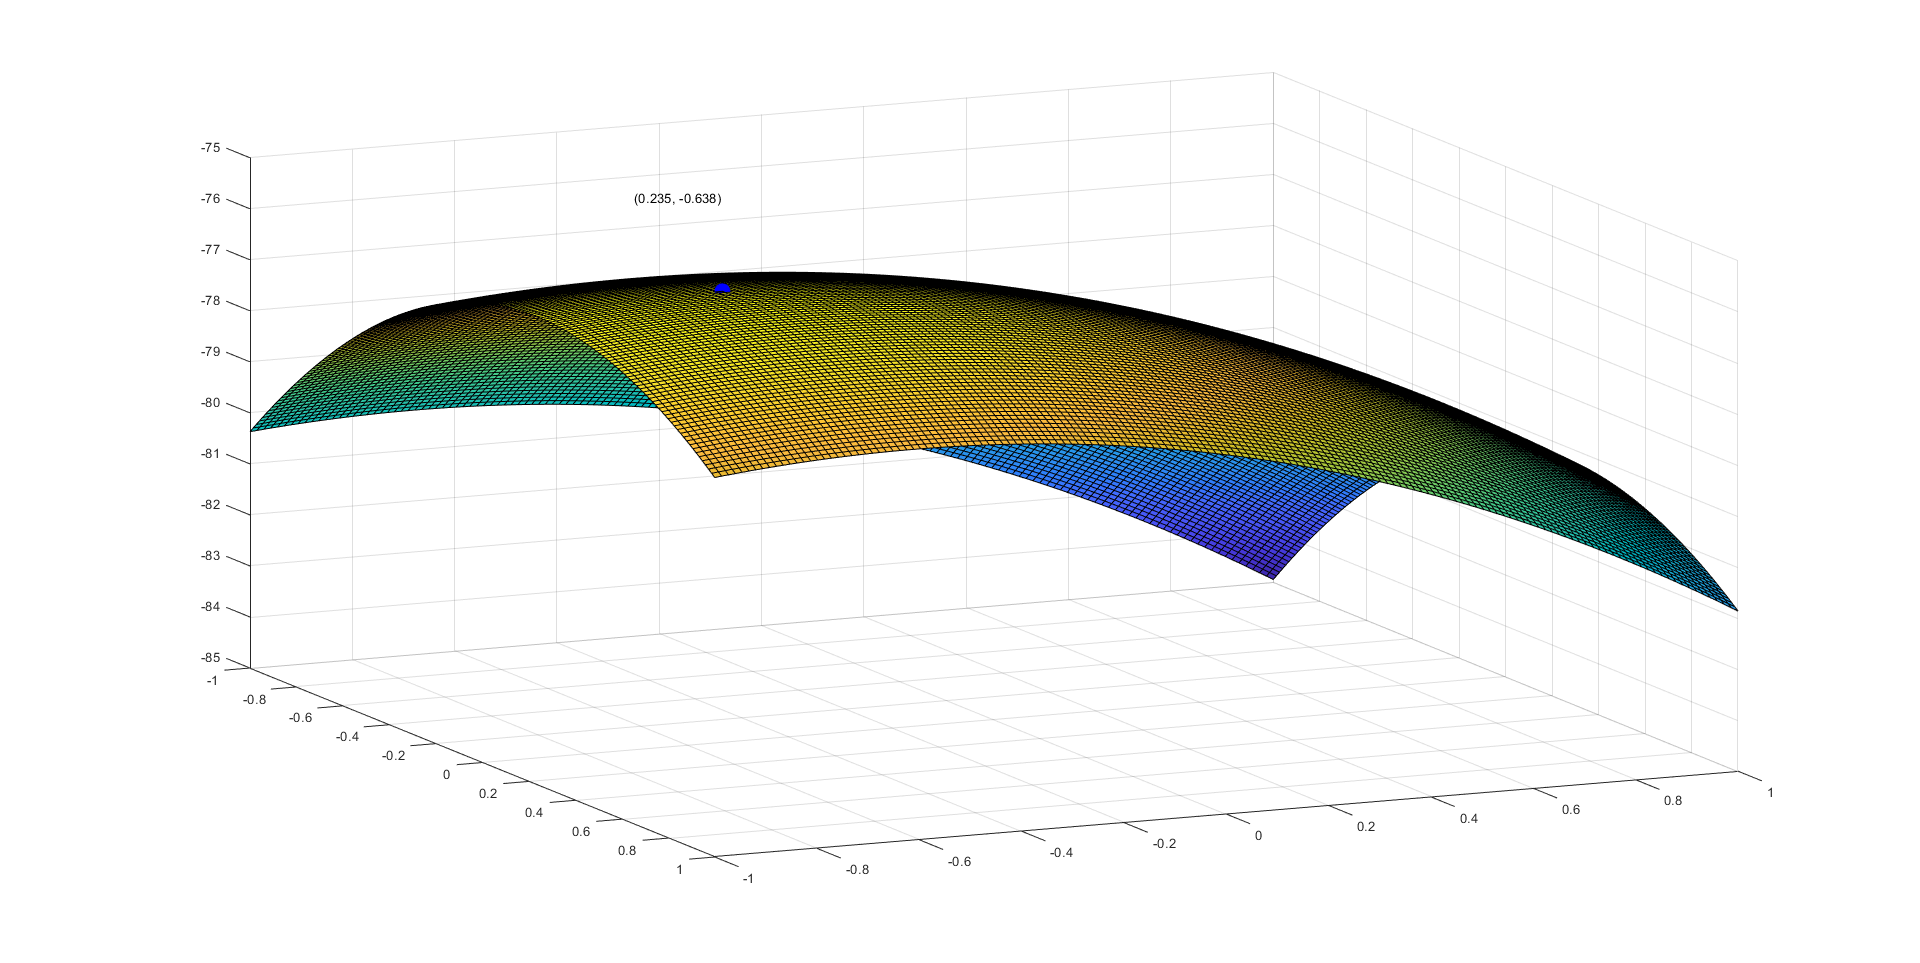
\includegraphics[scale=0.3]{./matlab/chapter-4/sol4.41.d.surf.png}
        \end{figure}
    \end{center}
\end{enumerate}